\documentclass[conference]{IEEEtran}
\IEEEoverridecommandlockouts

\usepackage{cite}
\usepackage{amsmath,amssymb,amsfonts}
\usepackage{algorithmic}
\usepackage{graphicx}
\usepackage{textcomp}
\usepackage{xcolor}
\usepackage{booktabs}

\def\BibTeX{{\rm B\kern-.05em{\sc i\kern-.025em b}\kern-.08em
    T\kern-.1667em\lower.7ex\hbox{E}\kern-.125emX}}

\begin{document}

\title{A Lightweight Noise-Robust Post-Trigger Classifier for Embedded Acoustic Artillery Launch Detection}

\author{
\IEEEauthorblockN{Martin Maxa}
\IEEEauthorblockA{
\textit{Czech Technical University in Prague,} \\
\textit{Faculty of Electrical Engineering} \\
Prague, Czech Republic \\
maxamart@fel.cvut.cz
}
\and
\IEEEauthorblockN{Jakub Svatos}
\IEEEauthorblockA{
\textit{Czech Technical University in Prague,} \\
\textit{Faculty of Electrical Engineering} \\
Prague, Czech Republic \\
svatoja1@fel.cvut.cz
}
\and
\IEEEauthorblockN{Jakub Zelinka}
\IEEEauthorblockA{
\textit{Czech Technical University in Prague,} \\
\textit{Faculty of Electrical Engineering} \\
Prague, Czech Republic \\
zelinjak@fel.cvut.cz
}
}

\maketitle

\begin{abstract}
Acoustic artillery sensing in the field must tolerate background noise while running on low-power embedded hardware. We study the post-trigger classification stage of a lightweight two-stage pipeline for artillery launch detection. The main corpus contains 706 clean labeled events: 62 artillery launches and 644 non-launch events. We train the classifier with an expanded non-launch corpus, class-imbalance mitigation, and train-time augmentation based on mel-frequency cepstral coefficient (MFCC)-domain perturbation. We evaluate the classifier under waveform-domain additive noise applied before MFCC extraction at acoustic signal-to-noise ratio (SNR) levels of 30, 20, 10, and 5~dB. On ESP32-S3 with TensorFlow Lite Micro, the deployed classifier preserves high performance under the tested conditions, with Matthews correlation coefficient (MCC) values of 0.99 at 30~dB and 0.80 at 5~dB. The experiment supports a lightweight embedded post-trigger classifier as part of a two-stage detection pipeline, although the robustness effect of quantization remains an empirical observation rather than a proven causal mechanism.
\end{abstract}

\begin{IEEEkeywords}
acoustic detection, artillery launch, MFCC, CNN, TensorFlow Lite, embedded AI, robustness, waveform-domain noise
\end{IEEEkeywords}

\section{Introduction}
Passive acoustic sensing can support early warning in contested environments where active systems are expensive, power-demanding, or easier to locate. Recent high-intensity conflicts have increased the need for low-cost passive systems that can detect artillery launches without emitting signals of their own. A practical acoustic system for this task must satisfy two constraints: (i) robustness to background noise and event variability and (ii) feasible execution on low-power embedded hardware.

Existing acoustic weapon-detection pipelines usually separate continuous-event triggering from the interpretation of short post-trigger signal windows. Triggering often relies on thresholding, energy-envelope analysis, time-of-arrival logic, or multi-sensor consistency checks. Post-trigger classification then uses engineered time-frequency or cepstral descriptors and, more recently, CNN-style classifiers~\cite{desai2005he_cb,hohil2007variants,piczak2015esc_cnn,svatos2024fcc}. For embedded artillery-launch sensing, the key question is whether a compact classifier trained with efficient MFCC-domain augmentation remains stable under waveform-domain additive noise and after quantized deployment on low-power hardware.

We adopt a two-stage processing architecture. A streaming trigger first identifies candidate impulsive events, and a post-trigger classifier then processes short acoustic segments. We treat the trigger, data acquisition, and circular-buffer logic as previously validated components and focus on the artillery launch classifier. Within this scope, we test whether a lightweight classifier preserves useful discrimination under controlled waveform-domain additive noise reported as acoustic signal-to-noise ratio (SNR) levels, while still fitting deployment on ESP32-S3.

Our training strategy combines an expanded non-launch corpus, class-imbalance mitigation, and train-time MFCC-domain augmentation. We evaluate whether this design maintains near-clean behavior when additive noise is applied to the waveform before MFCC extraction. We also assess whether the same classifier remains useful after quantization and deployment through TensorFlow Lite Micro on ESP32-S3, using PC-side 8-bit integer (int8) inference as the immediate reference point.

We frame artillery-launch sensing as a two-stage problem and focus the experiments on the post-trigger classifier. We evaluate the classifier on an expanded 706-event corpus under controlled waveform-domain additive noise, and we report ESP32-S3 deployment results together with PC-side int8 verification.

\section{State of the Art}
\subsection{Classical Acoustic Detection of Impulsive Events}
Weapon-related acoustic surveillance has traditionally used thresholding, energy-envelope analysis, time-of-arrival logic, and multi-sensor consistency checks to detect impulsive transients before semantic classification. Operational pipelines usually split artillery and gunshot processing into two tasks: (i) event triggering in continuous audio streams and (ii) post-trigger interpretation of short signal segments. Battlefield-oriented studies show that reliable operation depends on transient triggering that tolerates propagation distortion, changing stand-off distances, and heterogeneous sensor layouts~\cite{desai2005he_cb,desai2006launch_impact,hohil2007variants,dagallier2019long_range}. Trigger quality therefore limits downstream classifier performance.

\subsection{Acoustic Signature of Artillery and Gunfire}
Artillery and gunfire recordings do not follow a single invariant waveform. Source type, firing geometry, propagation, and local reflections shape each event. Depending on scenario and range, a recording may include different mixtures of muzzle blast, shock waves from supersonic projectiles, and delayed arrivals. Fig.~\ref{fig:artillery_long_waveform} shows an example artillery-launch waveform before extraction of the 60~ms post-trigger analysis window. Prior studies captured these effects indirectly through time-frequency or cepstral descriptors. Long-range studies modeled wave arrivals explicitly and documented sensitivity to atmosphere, terrain, and sensor geometry~\cite{desai2005he_cb,desai2006launch_impact,dagallier2019long_range}. These factors create domain shift: models tuned on narrow or clean recording conditions often degrade when transferred to field recordings with stronger multipath, clutter, and nonstationary background noise.

\begin{figure}[!tbh]
\centering
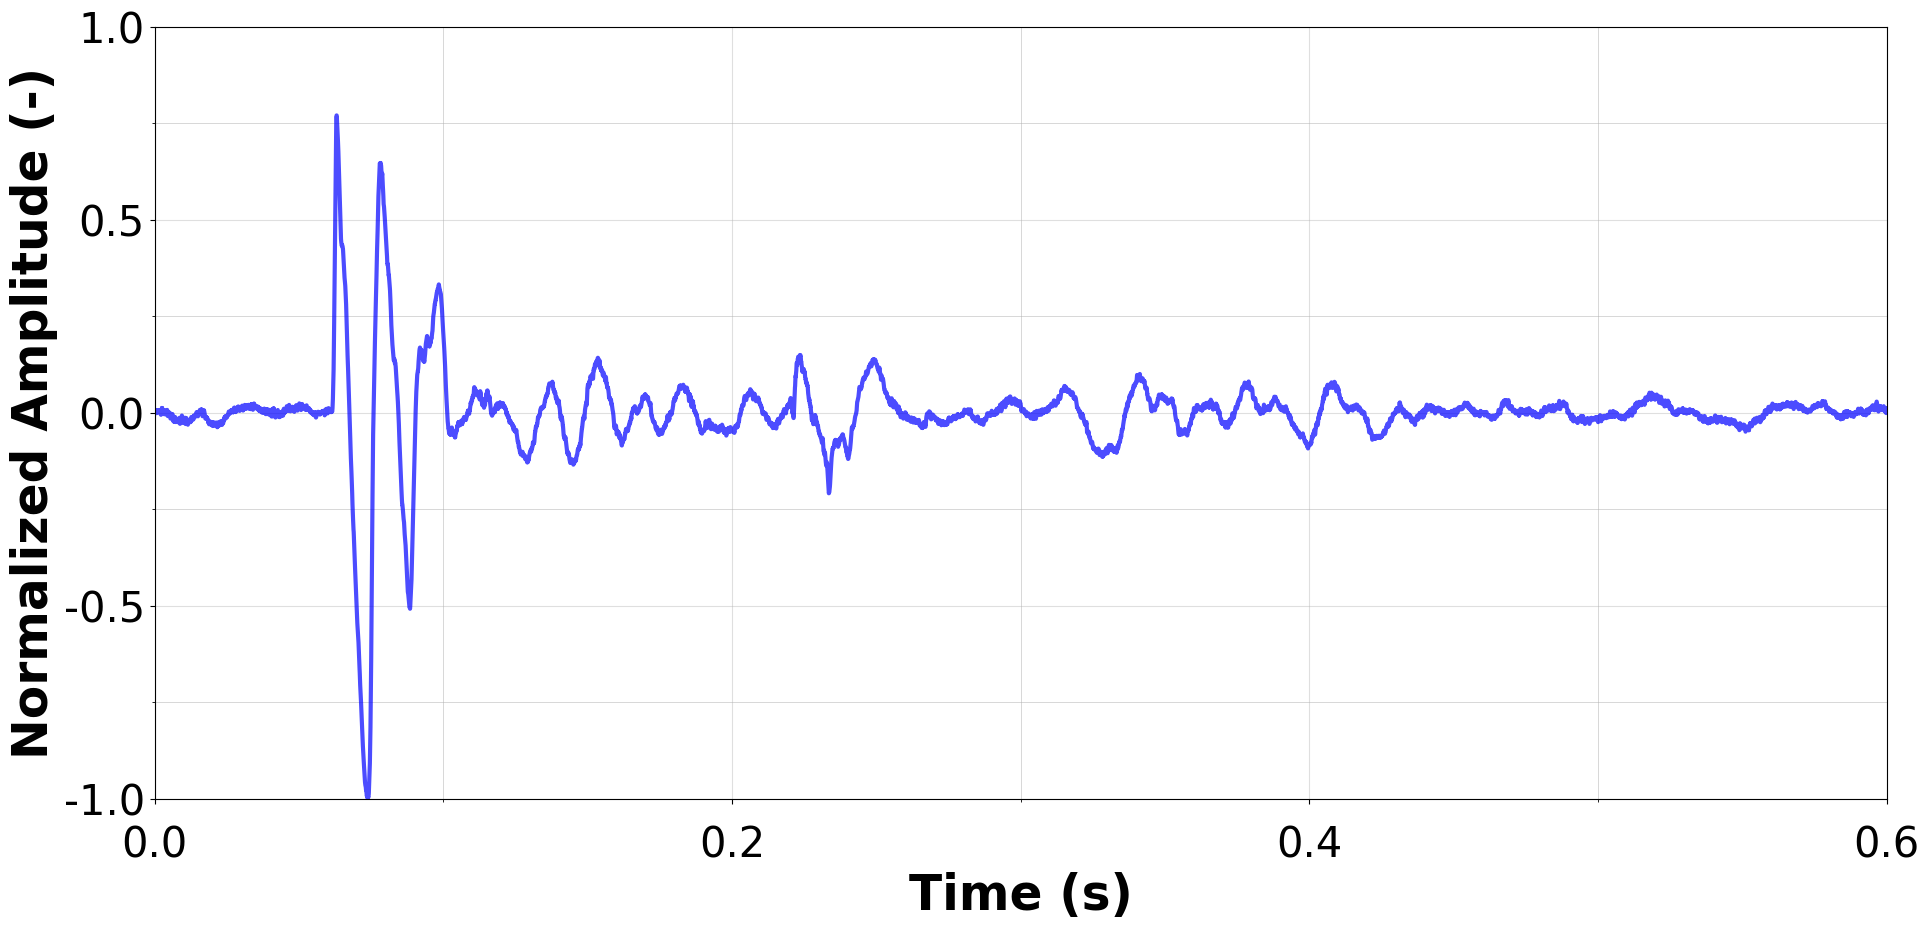
\includegraphics[width=\linewidth]{figs/sec2_artillery_waveform_plot_2.png}
\caption{Example artillery-launch waveform before extraction of the 60~ms post-trigger analysis window.}
\label{fig:artillery_long_waveform}
\end{figure}

\subsection{From Detection to Post-Detection Classification}
After trigger detection, systems usually classify short post-trigger windows. Classical approaches combine engineered representations, such as wavelet, cepstral, or temporal-envelope features, with shallow classifiers. Later methods use convolutional neural network (CNN) models over spectro-temporal inputs~\cite{hohil2007variants,khan2010embedding,raponi2022sound_of_guns,piczak2015esc_cnn,salamon2017esc_aug}. Cepstral representations remain attractive because they compactly encode the spectral envelope of short acoustic events~\cite{davis1980mfcc}. Broader environmental-sound evidence also shows that complementary time-frequency descriptors can matter when transient temporal structure is informative~\cite{chu2009env_sound_tf}. Comparative evidence from related gunshot-classification experiments suggests that performance depends on the interaction between the feature family and the classifier, not on model choice alone. In those comparisons, mel-frequency cepstral coefficient (MFCC)-based representations remained competitive against related cepstral alternatives for both neural and non-neural classifiers~\cite{svatos2024fcc}. These findings favor a two-stage design with a robust trigger and a compact post-trigger classifier. In a small-data embedded setting, a compact representation can be preferable to richer inputs when robustness and deployment cost must be balanced.

This motivates compact CNN topologies that preserve local time-frequency structure while remaining deployable on constrained hardware. A small stack of local convolutions, pooling, and a dense classification head follows the established LeNet-like pattern for compact two-dimensional inputs~\cite{lecun1998gradient}. In audio classification, analogous CNNs operate on time-frequency representations and learn local spectro-temporal patterns rather than hand-coded feature interactions~\cite{piczak2015esc_cnn,hershey2017cnn_audio}. For microcontroller-oriented deployments, this established small-footprint design logic is often preferable to deeper architectures when memory, latency, and operator support are limiting factors~\cite{banbury2021micronets}. In this work, we use a task-specific compact MFCC-CNN adapted to the $(58,12)$ input geometry and validate it as the second stage of the embedded artillery-launch pipeline.

\subsection{Robustness and Domain-Shift Handling}
Recent studies report strong performance under uncontrolled recording conditions, but many results remain tied to dataset-specific priors, acquisition pipelines, and label granularity~\cite{khan2010embedding,raponi2022sound_of_guns,svatos2024fcc}. In practice, model performance can degrade under perturbation, recording-device mismatch, changes in background scenes, or overlapping sound sources~\cite{ye2019multi_sound}. Clean-set accuracy alone is therefore insufficient. Augmentation strategy, perturbation tolerance, and operating-point calibration become central requirements~\cite{salamon2017esc_aug}. For embedded artillery-launch sensing, the relevant test is whether class separability survives waveform-domain additive noise before feature extraction, because this more closely follows the acoustic front-end encountered by a deployed system.

Feature-domain augmentation provides a relevant methodological precedent. SpecAugment, for example, applies warping and masking directly to log-mel feature inputs rather than to raw audio~\cite{park2019specaugment}. Similar feature-level Gaussian noise injection has also been used in noise-robust ASR, where artificial Gaussian noise is added to acoustic feature representations during training~\cite{braun2017accan}. Cepstral-domain processing has likewise been used for noise compensation in robust ASR~\cite{rehr2015cepstral_noise}. These precedents support treating MFCC space as a meaningful domain for efficient train-time regularization. At the same time, waveform-level additive noise and MFCC-domain additive perturbations are not equivalent, because additive noise before feature extraction produces nonlinear distortions in cepstral space~\cite{delatorre2002nonlinear_feature_space}. This distinction motivates our separation between MFCC-domain augmentation during training and waveform-domain noise during evaluation.

\subsection{Embedded Deployment and Runtime Constraints}
Edge deployment requires detection quality to be evaluated together with memory footprint, latency, and energy use. Tiny machine learning (TinyML) comparisons show that front-end feature extraction can dominate runtime, so the highest-accuracy model is not always the most deployable one~\cite{muthumala2024tinyml_ae}. Raspberry Pi and Tensor Processing Unit (TPU)-class studies further show that moderate accuracy loss may be acceptable when the system meets real-time constraints and resource budgets~\cite{lamrini2023embedded_esr}. MCU-focused TinyML systems also show that memory, latency, energy, and runtime overhead can dominate architecture and deployment choices on commodity microcontrollers~\cite{lin2020mcunet,banbury2021micronets}. Together with TensorFlow Lite deployment practice~\cite{tflite,david2021tflm} and integer or fixed-point quantization methods for efficient on-device inference~\cite{jacob2018quantization,benkhalifa2024stm32_quantization}, these findings motivate validation that separates desktop float32 behavior, quantized desktop verification, and embedded execution.

We therefore address a narrower question than full continuous surveillance: whether a lightweight post-trigger classifier for artillery launch sensing remains robust under controlled perturbation and maintains performance after quantized deployment on an embedded target.

\section{Method}
\subsection{Processing Pipeline}
We study the post-trigger classification stage of a two-stage acoustic pipeline. In the full architecture, the first stage follows a median-filter impulse-detection approach: a streaming trigger estimates the local acoustic background, identifies candidate impulsive events, and forwards short buffered segments to a classifier~\cite{svatos2019smart_acoustic_sensor}. The trigger, acquisition chain, and online buffering logic are outside the scope of this study and are treated as previously validated components. We evaluate only the second stage, the post-trigger CNN artillery launch classifier.

Each candidate event is represented by a 60~ms waveform segment centered on the detected impulse peak. The segment is asymmetric: 40~\% precedes the peak to capture onset structure, and 60~\% follows it to retain decay and muzzle-blast content. Fig.~\ref{fig:artillery_waveform} shows an example of the resulting waveform segment. We then compute MFCC features from these segments for supervised CNN training and inference.

\begin{figure}[!tbh]
\centering
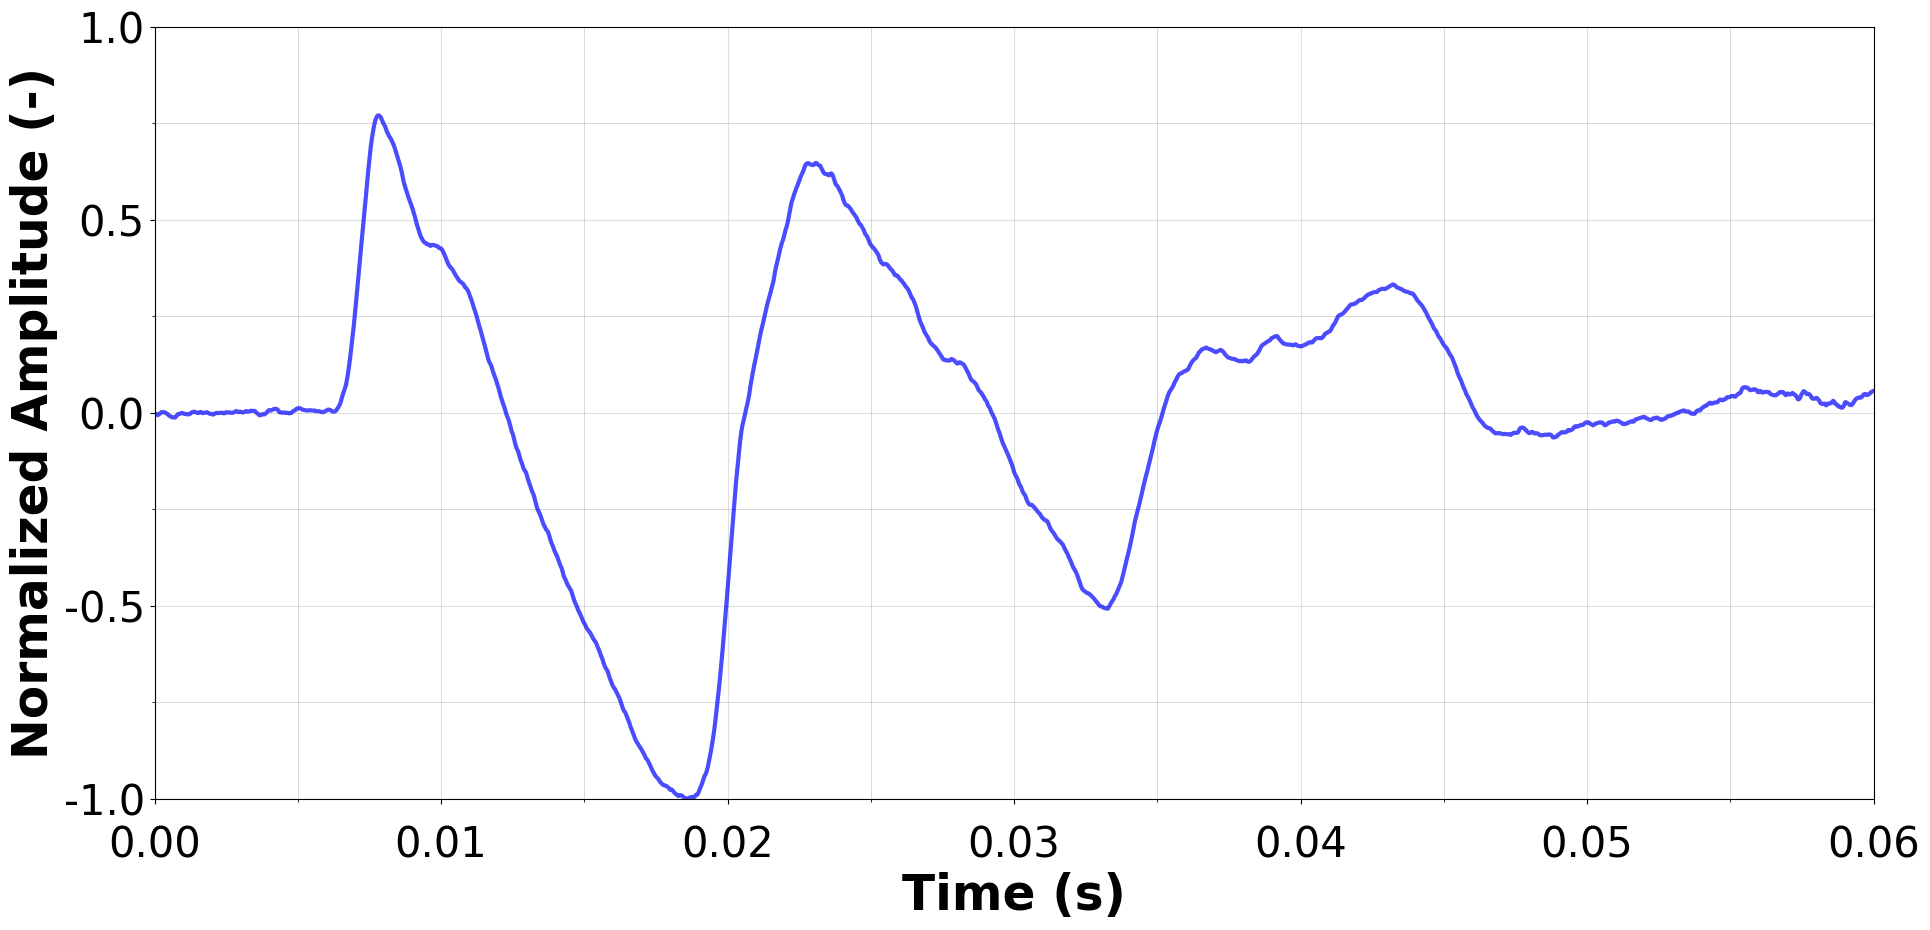
\includegraphics[width=\linewidth]{figs/sec3_artillery_cropped_60ms_2.png}
\caption{Example 60~ms peak-centered waveform segment used for MFCC extraction.}
\label{fig:artillery_waveform}
\end{figure}

\subsection{Field Data Acquisition}
The source corpus comes from real artillery measurements and includes both launch and impact acoustic events. We collected the recordings with the field station shown in Fig.~\ref{fig:recording_station}. The acquisition chain used PreSonus PRM1 microphones connected through a Roland Rubix 44 audio interface, and the signal processing uses 16-bit audio at 22.05~kHz. We model only binary artillery launch classification (artillery launch vs. non-launch) and leave impact-event modeling for future work. The positive class contains only artillery launch events, whereas the non-launch class contains impulsive false-trigger candidates, including door impacts, human shouts, bell sounds, small-arms gunshots, and other impulsive non-artillery recordings.

The main clean corpus contains 706 labeled events, summarized in Table~\ref{tab:dataset_overview}. We expanded the non-launch class to better reflect operational negatives and to strengthen training under perturbation.

\begin{table}[!tbh]
\caption{Overview of labeled acoustic events}
\label{tab:dataset_overview}
\centering
\scriptsize
\begin{tabular}{@{}lcc@{}}
\toprule
Subset & Events & Share \\
\midrule
Artillery launch & 62 & 8.8~\% \\
Non-launch & 644 & 91.2~\% \\
Main clean corpus & 706 & 100~\% \\
\bottomrule
\end{tabular}
\end{table}

\begin{figure}[!tbh]
\centering
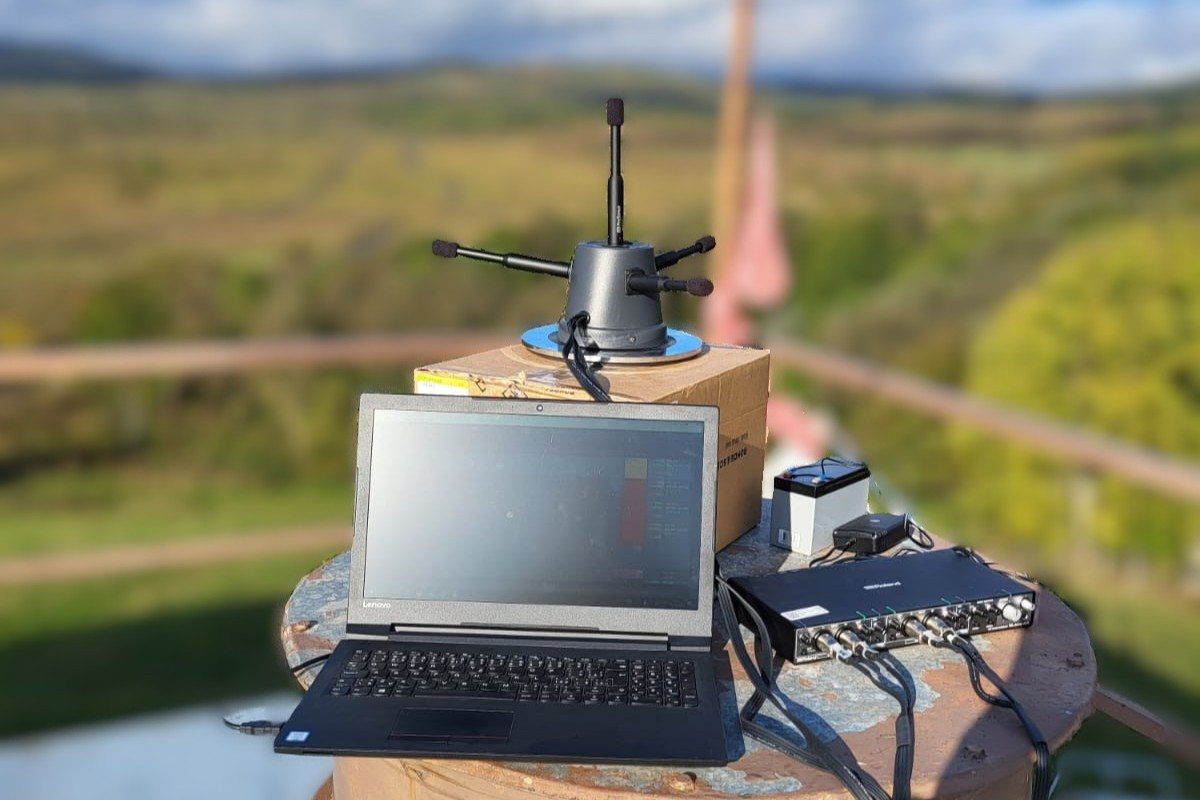
\includegraphics[width=\linewidth]{figs/sec2_measuring_setup.jpg}
\caption{Field recording station used for artillery dataset acquisition.}
\label{fig:recording_station}
\end{figure}

\subsection{CNN Topology}
The network input is an MFCC tensor of size $(58,12,1)$ in \texttt{channels\_last} format. The classifier first applies a valid Conv2D layer with 32 filters, a $3\times3$ kernel, stride 1, and rectified linear unit (ReLU) activation, producing a $(56,10,32)$ tensor. A $2\times2$ MaxPooling2D layer with stride 2 reduces this representation to $(28,5,32)$. The second valid Conv2D layer uses 64 filters with the same $3\times3$ kernel, stride 1, and ReLU activation, producing $(26,3,64)$. A second $2\times2$ MaxPooling2D layer with stride 2 then yields $(13,1,64)$. The result is flattened to 832 features, passed through Dense(64) with ReLU, regularized by Dropout(0.5), and classified by a final Dense(1) sigmoid output. The trainable parameter counts are 320 for the first convolution, 18,496 for the second convolution, 53,312 for Dense(64), and 65 for the output layer, for a total of 72,193 trainable parameters; the pooling, flattening, and dropout layers add no trainable parameters. Fig.~\ref{fig:cnn_architecture} shows the full architecture. We train the final model for 50 epochs with the Adam optimizer and binary cross-entropy loss. This layout balances representation capacity and deployment cost, following standard convolutional design practice~\cite{lecun1998gradient}.

\begin{figure}[!tbh]
\centering
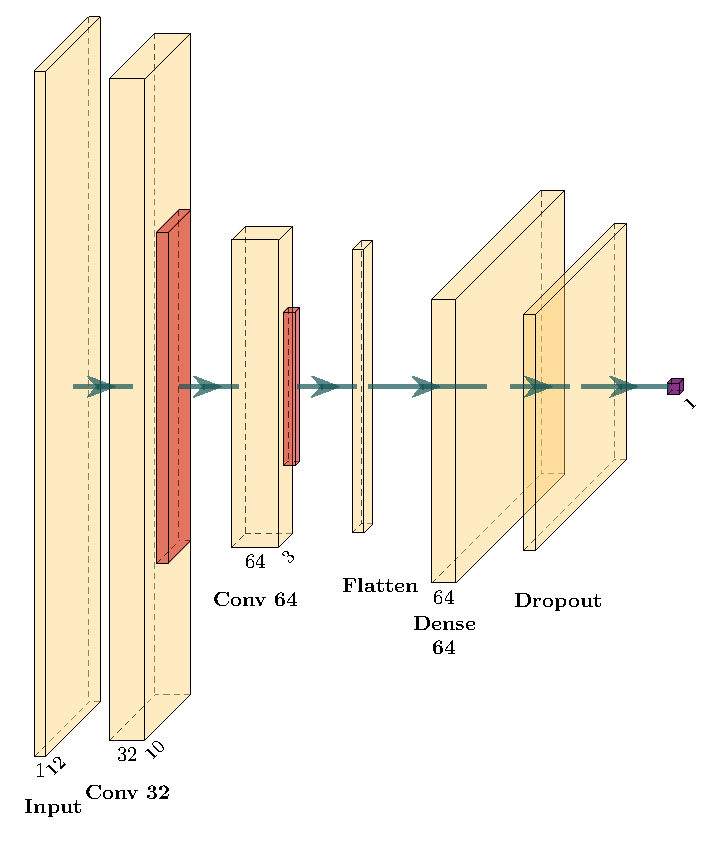
\includegraphics[width=0.75\linewidth]{figs/sec3_cnn_architecture.pdf}
\caption{CNN topology used for post-trigger artillery launch classification of MFCC segments.}
\label{fig:cnn_architecture}
\end{figure}

\subsection{Robustness Training}
We extract MFCCs from 22.05~kHz signals using short-time framing with high temporal resolution. Each 60~ms segment is divided into 2.5~ms frames (approximately 55 samples) with a 1.0~ms hop (approximately 22 samples), corresponding to 1.5~ms overlap (60~\%). A Hamming window is applied to each frame to reduce spectral leakage, and the spectrum is evaluated with a 512-point fast Fourier transform ($NFFT=512$). The mel front end uses 40 mel filters, from which the first 12 MFCC coefficients are retained. This yields the $(58,12,1)$ input tensor used by the classifier.

The training strategy combines three elements: (i) an expanded non-launch corpus, (ii) class-imbalance mitigation, and (iii) train-time augmentation of the training split only. This follows the broader use of augmentation for audio classification under limited-data conditions~\cite{salamon2017esc_aug}. Gaussian perturbations are applied directly to the precomputed MFCC matrices as a feature-space input-noise regularization strategy. Since the CNN receives MFCC tensors as its input, this perturbation acts on the representation seen by the network and encourages stable predictions for locally perturbed cepstral representations. Training with input noise is theoretically related to Tikhonov regularization~\cite{bishop1995training_noise}, and feature-level Gaussian noise injection has also been used in noise-robust ASR~\cite{braun2017accan}. This MFCC-domain feature jittering is used for efficient training augmentation only. The robustness results below use a separate waveform-domain evaluation protocol in which additive Gaussian noise is applied to the audio signal before MFCC extraction. Additive waveform noise passes through STFT magnitude computation, mel-filterbank integration, logarithmic compression, and DCT, producing a nonlinear cepstral distortion rather than a simple additive MFCC offset~\cite{delatorre2002nonlinear_feature_space}.

\subsection{Imbalance and Overfitting Mitigation}
Because the corpus is strongly imbalanced, with artillery-launch events representing only about 8.8~\% of the 706 labeled samples, training uses class-weighted optimization to reduce majority-class bias, following standard imbalanced-learning practice~\cite{he2009imbalanced}. The loss assigns a stronger penalty to errors on the minority artillery-launch class, so high nominal accuracy cannot be achieved simply by collapsing predictions toward the majority non-launch class. Class weighting is therefore included in the final training configuration.

\subsection{Embedded Inference Protocol}
After PC training, we export the selected model to TensorFlow Lite Micro~\cite{tflite,david2021tflm}. To separate hardware effects from quantization effects, we evaluate three inference regimes: desktop float32 inference, desktop int8 inference with the quantized model, and ESP32-S3 deployment of the same quantized classifier. The embedded implementation uses int8 inference on ESP32-S3 with a statically allocated 80~KiB \texttt{tensor\_arena} for intermediate tensors and a selective \texttt{MicroMutableOpResolver} configuration that registers only the operators required by the network. This static-arena and selective-operator design follows the MCU-oriented TensorFlow Lite Micro runtime model. Int8 inference follows standard integer-only practice for reducing memory footprint and enabling efficient execution on resource-constrained processors~\cite{jacob2018quantization,david2021tflm}. Embedded validation uses a host-device protocol: the host generates waveform-domain noisy test variants, computes MFCC tensors from those modified waveforms, transmits the tensors to the embedded target, and collects predicted labels and scores. The ESP32-S3 experiment therefore validates the deployed TFLite Micro classifier only; MFCC extraction is performed on the host PC, and the reported latency corresponds to classifier inference on one MFCC segment, not to the complete audio acquisition, triggering, feature extraction, and classification pipeline. This host-device transfer is a validation protocol rather than the intended operational pipeline. We use ESP32-S3 as a representative low-power Edge AI platform for classifier deployment, not as a proof of universal generalization across embedded hardware.

\section{Experimental Setup}
The main dataset contains 706 clean labeled events: 62 artillery launches and 644 non-launch events. Model development used a stratified event-level 80/20 split, and train-time MFCC-domain augmentation was applied only to the training partition to prevent leakage between original events and their augmented variants. After selecting the final model, waveform-domain robustness was evaluated as a corpus-level stress test on the full 706-event corpus. For each acoustic SNR level of 30, 20, 10, and 5~dB, one noisy waveform variant was generated from each original event by adding scaled Gaussian noise before MFCC extraction. We report accuracy, precision, recall, F1-score, and Matthews correlation coefficient (MCC) using a fixed sigmoid decision threshold of 0.5. The robustness tables should therefore be interpreted as perturbation stress-test results for the selected model, not as independent hold-out generalization estimates. We compare:
\begin{enumerate}
\item desktop float32 post-trigger classification under waveform-domain additive noise,
\item PC-side int8 verification of the quantized model, and
\item ESP32-S3 deployment of the same quantized post-trigger classifier.
\end{enumerate}

\section{Results}
\subsection{Desktop Float32 Reference Under Waveform-Domain Noise}
Table~\ref{tab:pc_float32} summarizes the desktop float32 reference for the corpus-level waveform-domain robustness stress test. The model retains high recall across all tested SNR levels, but precision is low and degrades further under heavier corruption. As a result, MCC remains moderate and declines from 0.54 at 30~dB to 0.46 at 5~dB. The float32 reference therefore fails mainly through false-positive inflation rather than missed artillery launches.

\begin{table}[!tbh]
\caption{Desktop float32 robustness under waveform-domain additive noise.}
\label{tab:pc_float32}
\centering
\resizebox{\linewidth}{!}{%
\begin{tabular}{@{}cccccc@{}}
\toprule
SNR (dB) & Accuracy (\%) & Precision & Recall & F1-score & MCC \\
\midrule
30 & 84.41 & 0.35 & 1.00 & 0.52 & 0.54 \\
20 & 82.86 & 0.33 & 1.00 & 0.49 & 0.54 \\
10 & 81.12 & 0.31 & 0.99 & 0.47 & 0.49 \\
5  & 80.44 & 0.29 & 0.93 & 0.45 & 0.46 \\
\bottomrule
\end{tabular}
}
\end{table}

\subsection{PC-Side int8 Verification}
To separate hardware effects from quantization effects, we evaluate the quantized model on PC before moving to the embedded target. The PC-side int8 results in Table~\ref{tab:quantized_compare} are consistently stronger than the float32 reference under the same waveform-domain stress-test protocol, with MCC values of 0.92 at 30~dB and 0.65 at 5~dB. This intermediate step supports the interpretation that int8 quantization is associated with the robustness improvement observed later on the embedded target, although we do not isolate the exact mechanism from all preprocessing and deployment-related factors.

\subsection{ESP32-S3 Deployment Results}
Table~\ref{tab:quantized_compare} also reports the embedded ESP32-S3 results for the same quantized classifier under the waveform-domain stress-test protocol. In this setup, the embedded target attains MCC values from 0.99 at 30~dB to 0.80 at 5~dB. The average classifier inference latency per MFCC segment is approximately 32~ms, and the deployed implementation uses an 80~KiB \texttt{tensor\_arena}. These results indicate that the quantized post-trigger classifier remains deployable on the target platform under the tested host-device validation protocol.

\begin{table}[!tbh]
\caption{Quantized inference comparison under waveform-domain additive noise.}
\label{tab:quantized_compare}
\centering
\resizebox{\linewidth}{!}{%
\begin{tabular}{@{}ccccccc@{}}
\toprule
Mode & SNR (dB) & Accuracy (\%) & Precision & Recall & F1-score & MCC \\
\midrule
PC int8 & 30 & 98.66 & 0.86 & 1.00 & 0.93 & 0.92 \\
PC int8 & 20 & 96.77 & 0.72 & 1.00 & 0.84 & 0.83 \\
PC int8 & 10 & 92.74 & 0.54 & 0.97 & 0.69 & 0.69 \\
PC int8 & 5  & 92.41 & 0.53 & 0.90 & 0.66 & 0.65 \\
\midrule
ESP32-S3 & 30 & 99.86 & 1.00 & 0.98 & 0.99 & 0.99 \\
ESP32-S3 & 20 & 99.73 & 0.98 & 0.98 & 0.98 & 0.98 \\
ESP32-S3 & 10 & 97.78 & 0.86 & 0.87 & 0.87 & 0.86 \\
ESP32-S3 & 5  & 97.18 & 0.95 & 0.70 & 0.81 & 0.80 \\
\bottomrule
\end{tabular}
}
\end{table}

\section{Discussion and Limitations}
The experiment isolates the second stage of the pipeline: data acquisition and trigger generation provide candidate events, and the post-trigger classifier assigns the launch/non-launch label. The float32 desktop reference is not a sufficient proxy for embedded performance under waveform-domain additive noise. Quantized inference, first verified on PC and then deployed on ESP32-S3, stays more stable under the tested acoustic SNR levels.

The study has several limits. We do not evaluate continuous-stream trigger performance or false-trigger rates, so the system-level claim is limited to post-trigger classification. Model development used a single stratified event-level split, while the reported waveform-domain robustness results are corpus-level stress tests over all 706 labeled events. These results quantify perturbation stability of the selected model on the available corpus rather than independent repeated-split or session-independent generalization. The noise study uses synthetic additive Gaussian noise in the waveform domain; this is closer to the deployed acoustic front end than MFCC-domain perturbation, but it still omits many field-noise, propagation, and recording-device shifts. The apparent robustness benefit associated with quantization is an empirical observation supported by the PC-side int8 bridge experiment, not an isolated mechanistic proof. One plausible explanation is that int8 quantization suppresses small MFCC-level variations introduced by waveform-domain noise after nonlinear feature extraction; however, preprocessing, scaling, thresholding, and runtime-specific numerical details were not independently ablated. The corpus also remains small in positive artillery-launch events, and the deployment study validates the ESP32-S3 classifier rather than a complete on-device audio-to-decision pipeline.

\section{Conclusion}
We presented a lightweight two-stage acoustic pipeline for embedded artillery launch detection and evaluated its post-trigger classification stage under waveform-domain additive noise applied before MFCC extraction. The classifier uses a compact LeNet-like MFCC-CNN architecture designed to provide a small-footprint second-stage model that is simple enough for MCU deployment while still retaining useful discrimination under controlled acoustic degradation.

On the expanded 706-event corpus, the desktop float32 reference remains vulnerable to false positives, whereas quantized inference is more robust under the tested waveform-domain SNR levels. PC-side int8 verification and ESP32-S3 deployment show that the post-trigger classifier can run on the target platform under the host-device validation protocol, reaching MCC values of 0.99 at 30~dB and 0.80 at 5~dB with approximately 32~ms average classifier inference latency per MFCC segment and an 80~KiB \texttt{tensor\_arena}.

Within the stated scope, the results support the feasibility of an embedded post-trigger artillery-launch classifier. The main contribution is the embedded validation of a practical second-stage classifier built around a task-specific lightweight MFCC-CNN under controlled waveform-domain perturbations. Future work should extend the validation to continuous-stream false-trigger rates, on-device MFCC extraction, end-to-end latency, more diverse field-noise conditions, repeated-split or session-independent uncertainty estimation, and broader deployment targets.

\bibliographystyle{IEEEtran}
\bibliography{references}

\end{document}
